%% This is file `elsarticle-template-1-num.tex',
%%
%% Copyright 2009 Elsevier Ltd
%%
%% This file is part of the 'Elsarticle Bundle'.
%% ---------------------------------------------
%%
%% It may be distributed under the conditions of the LaTeX Project Public
%% License, either version 1.2 of this license or (at your option) any
%% later version.  The latest version of this license is in
%%    http://www.latex-project.org/lppl.txt
%% and version 1.2 or later is part of all distributions of LaTeX
%% version 1999/12/01 or later.
%%
%% The list of all files belonging to the 'Elsarticle Bundle' is
%% given in the file `manifest.txt'.
%%
%% Template article for Elsevier's document class `elsarticle'
%% with numbered style bibliographic references
%%
%% $Id: elsarticle-template-1-num.tex 149 2009-10-08 05:01:15Z rishi $
%% $URL: http://lenova.river-valley.com/svn/elsbst/trunk/elsarticle-template-1-num.tex $
%%
\documentclass[preprint,12pt]{elsarticle}
\usepackage{amsmath}
\usepackage{graphicx,subcaption}
\usepackage{listings}
\usepackage{hyperref}
\usepackage{multirow}
\usepackage{notoccite}
\hypersetup{
    colorlinks,
    citecolor=black,
    filecolor=black,
    linkcolor=black,
    urlcolor=black
}

%% Use the option review to obtain double line spacing
%% \documentclass[preprint,review,12pt]{elsarticle}

%% Use the options 1p,twocolumn; 3p; 3p,twocolumn; 5p; or 5p,twocolumn
%% for a journal layout:
%% \documentclass[final,1p,times]{elsarticle}
%% \documentclass[final,1p,times,twocolumn]{elsarticle}
%% \documentclass[final,3p,times]{elsarticle}
%% \documentclass[final,3p,times,twocolumn]{elsarticle}
%% \documentclass[final,5p,times]{elsarticle}
%% \documentclass[final,5p,times,twocolumn]{elsarticle}

%% if you use PostScript figures in your article
%% use the graphics package for simple commands
%% \usepackage{graphics}
%% or use the graphicx package for more complicated commands
%% \usepackage{graphicx}
%% or use the epsfig package if you prefer to use the old commands
%% \usepackage{epsfig}

%% The amssymb package provides various useful mathematical symbols
\usepackage{amssymb}
%% The amsthm package provides extended theorem environments
%% \usepackage{amsthm}

%% The lineno packages adds line numbers. Start line numbering with
%% \begin{linenumbers}, end it with \end{linenumbers}. Or switch it on
%% for the whole article with \linenumbers after \end{frontmatter}.
\usepackage{lineno}

%% natbib.sty is loaded by default. However, natbib options can be
%% provided with \biboptions{...} command. Following options are
%% valid:

%%   round  -  round parentheses are used (default)
%%   square -  square brackets are used   [option]
%%   curly  -  curly braces are used      {option}
%%   angle  -  angle brackets are used    <option>
%%   semicolon  -  multiple citations separated by semi-colon
%%   colon  - same as semicolon, an earlier confusion
%%   comma  -  separated by comma
%%   numbers-  selects numerical citations
%%   super  -  numerical citations as superscripts
%%   sort   -  sorts multiple citations according to order in ref. list
%%   sort&compress   -  like sort, but also compresses numerical citations
%%   compress - compresses without sorting
%%
%% \biboptions{comma,round}

% \biboptions{}

\let\originaleqref\eqref
\renewcommand{\eqref}{Eq.~\originaleqref}

\hypersetup{colorlinks=true,
  pdftitle={Performance and Accuracy of WARP - A Framework for Continuous Energy Monte Carlo Neutron Transport in General 3D Geometries on GPUs},
  pdfauthor={Ryan M. Bergmann, Kelly Rowland, Nikola Radnovi\'c, Jasmina L. Vuji\'c}}

\journal{Annals of Nuclear Energy}

\begin{document}

\begin{frontmatter}

%% Title, authors and addresses

%% use the tnoteref command within \title for footnotes;
%% use the tnotetext command for the associated footnote;
%% use the fnref command within \author or \address for footnotes;
%% use the fntext command for the associated footnote;
%% use the corref command within \author for corresponding author footnotes;
%% use the cortext command for the associated footnote;
%% use the ead command for the email address,
%% and the form \ead[url] for the home page:
%%
%% \title{Title\tnoteref{label1}}
%% \tnotetext[label1]{}
%% \author{Name\corref{cor1}\fnref{label2}}
%% \ead{email address}
%% \ead[url]{home page}
%% \fntext[label2]{}
%% \cortext[cor1]{}
%% \address{Address\fnref{label3}}
%% \fntext[label3]{}

\title{Performance and Accuracy of WARP - A Framework for Continuous Energy Monte Carlo Neutron Transport in General 3D Geometries on GPUs}

%% use optional labels to link authors explicitly to addresses:
%% \author[label1,label2]{<author name>}
%% \address[label1]{<address>}
%% \address[label2]{<address>}

\author{Ryan M. Bergmann \corref{rmb}}
\ead{ryanmbergmann@gmail.com}
\cortext[rmb]{Corresponding author. Tel.: +41.76.687.53.09.}

\author{Kelly Rowland }
\ead{krowland@berkeley.edu}

\author{Nikola Radnovi\'c }
\ead{radnovicn@gmail.com}

\author{Jasmina L. Vuji\'c }
\ead{vujic@nuc.berkeley.edu}


\address{Department of Nuclear Engineering, 
4155 Etcheverry Hall, 
University of California - Berkeley,
Berkeley, CA 94703-1730}

\begin{abstract}

In this companion paper to ``Algorithmic Choices in WARP - A Framework for Continuous Energy Monte Carlo Neutron Transport in General 3D Geometries on GPUs'' (doi:10.1016/j.anucene.2014.10.039), the WARP Monte Carlo neutron transport framework for GPUs is benchmarked against production-level CPU Monte Carlo neutron transport codes for both performance and accuracy.  Fission source distributions, flux spectra, and multiplication factors calculated by WARP are compared to those from Serpent v2.XX.X and MCNP v6.1. for identical materials and geometries.  Runtimes are also reported.

\end{abstract}

\begin{keyword}
Monte Carlo \sep Neutron Transport \sep GPU \sep CUDA \sep CUDPP \sep OptiX


\end{keyword}

\end{frontmatter}

\linenumbers

%% main text

\section{Introduction}
\label{sec:intro}

Developing WARP was motivated by modern supercomputers commonly being built with graphics processing units (GPU) coprocessor cards in their nodes to increase their computational efficiency and performance \cite{}.  Compared to more common central processing units, or CPUs, GPUs have a larger aggregate memory bandwidth, much larger rate of floating-point operations per second (FLOPS), and lower energy consumption per FLOP\cite{}.  GPUs execute efficiently on data-parallel problems \cite{}, and since most CPU codes are task-parallel, the algorithms used had to be reconsidered.  Data-parallelism is simply parallelism that arises from operating on many different pieces of data at one time, whereas task-parallelism is parallelism that arises from running many concurrent tasks at one time which act on a single piece of data.   Figure \ref{datavtask} shows and illustration of the difference between a data-parallel and a task-parallel neutron transport loop.

\begin{figure}[h!] 
  \centering
    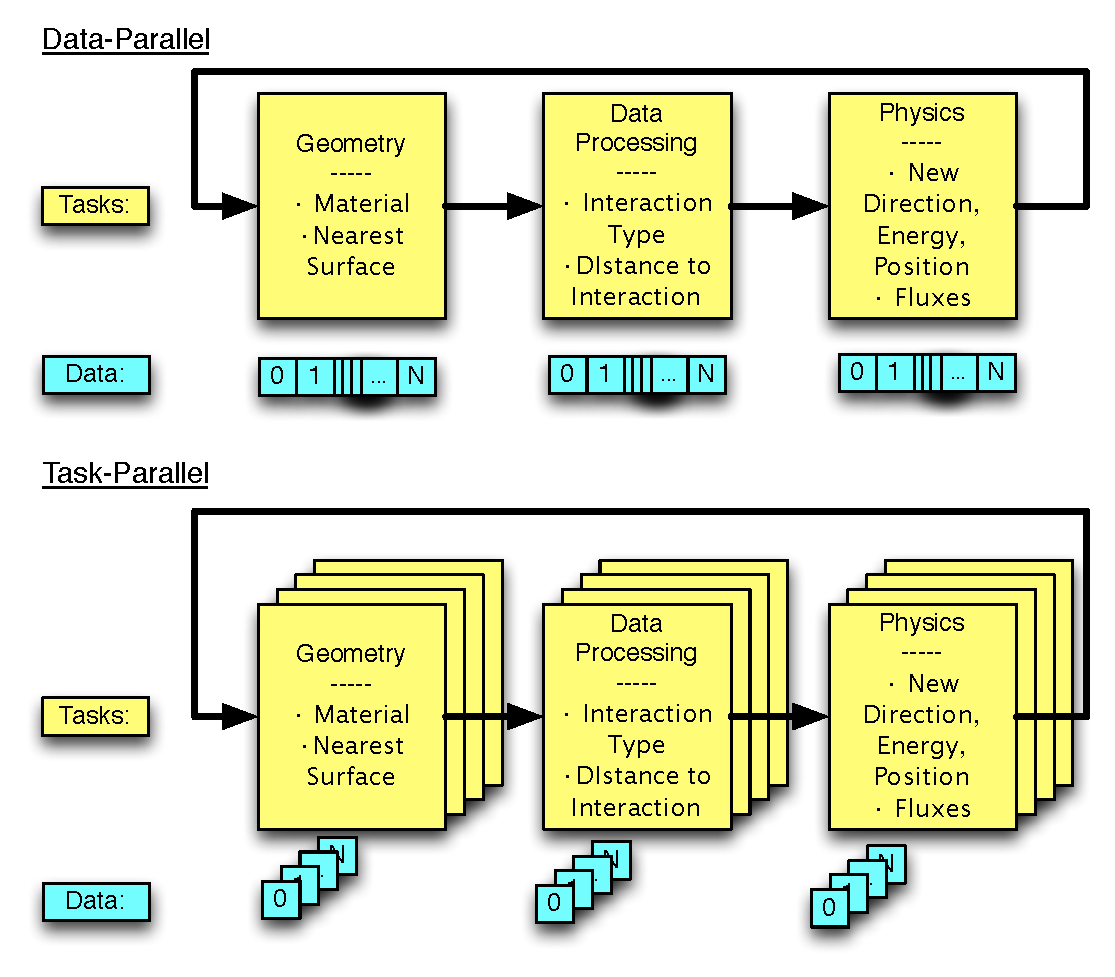
\includegraphics[width=\textwidth]{graphics/datavtask.pdf}
     \caption{Data-parallel neutron trasport loop vs. a task-parallel transport loop for N neutrons in parallel.  \label{datavtask} }
\end{figure}

Execution on GPUs also requires additional data management, since the on-chip memory of the GPU is separate from the host CPUs memory \cite{cuda}.  Execution on NVIDIA GPUs also required code to be written in CUDA, which is a set of extensions for C/C++.  The simplest way to accommodate all these requirements was to write a new code from scratch, which ultimately resulted in WARP.  

In this paper, results calculated by WARP are compared against those calculated by Serpent 2.XX.X and MCNP 6.1, two widely-used production-level Monte Carlo neutron transport codes, in order to ensure the accuracy of WARP and to highlight its performance differences.  The details about the algorithms used in WARP are discussed in \cite{algorithms}.


%%%%%%%%%%%%%%%%%%%
%%%%%%%%%%%%%%%%%%%
%%%%%%%%%%%%%%%%%%%
\section{Features of WARP}
\label{sec:features}

WARP has only existed since 2013, and is not as fully-featured as more mature Monte Carlo codes.  It has the functionality necessary to compare its performance against  Serpent 2.XX.X and MCNP 6.1, but there are many areas where feature need to be added in order for WARP to become a useful engineering and scientific tool.  This section outlines the current set of features available in WARP.  

\subsection{Physics}

Cross section data compiled by the United States is distributed by the Department of Energy in \emph{ENDF} files.  ENDF stands for ``evaluated nuclear data file,'' and can contain data for nuclear decay, photons, atomic relaxation, fission yields, thermal neutron scattering, and charged particle reactions as well as neutron reactions.  The data files are called ``evaluated'' because a group of experts decides, or evaluates, what data is included in them.  The data includes theoretical calculations of cross sections based on well developed models as well as experimental data.  They also decide how to represent regimes that haven't been measured yet by comparing simulation results to experiments.   The first data released was ENDF/B-I in 1968 and the latest set is ENDF/B-VII, which was released in 2006.  

The data is written in a standard format that dates back to when the data was stored on magnetic tapes, and data entries are sometimes referred to as ``tapes'' to this day.  The format is rather archaic and contains a lot of redundant information about record locations, which was useful when the tape head had to physically move between points in the tape \cite{endfnums}.  

Many Monte Carlo codes read ACE-formatted data rather than the original ENDF file.  ENDF files contain a lot of data so the dataset preserves the original evaluation, but most transport codes need the data in tabular format.  This is why transport codes normally use ACE-formatted data files. \cite{jaakko}  ACE stands for ``a compact ENDF'' and strips out a lot of the extra information unnecessary for neutron transport.  ENDF tapes contain information that is valuable for charged particles and photons as well as neutrons, and this information is discarded for neutron transport. As Figure \ref{data_levels} shows, ACE files not only contain cross sections, but also angle and energy distributions used in scattering and fission.  ENDF assigns a number to each type of reaction called the \emph{MT} number.  Table \ref{MT_numbers} in Appendix B, taken from a LANL website, shows what these MT numbers mean \cite{endfnums}.  

It can clearly be seen that there are many reactions a neutron can undergo, most of which have very strong energy dependence.  Most of the complexity in modeling nuclear reactors comes from the fact that the data needed to model neutrons is very complicated.  Data may be the most important part of the simulation; it is what ties the calculations to reality.  

ACE data files typically come pre-processed at different temperatures.  This processing can done by a code called NJOY \cite{jaakko}, which Doppler broadens all the resonances in the cross sections and adjusts the unresolved resonance tables accordingly.  It can also thin the energy grid if requested by the user, though this reduces the accuracy of the cross sections \cite{jaakko}.  Thinning the energy grid is a computationally intensive task, and NJOY is not parallelized.  Most production codes come with their own pre-processed datasets at several temperature intervals in order to save the user the time and effort needed to process data from ENDF files.






only neutrons of course, no photons, etc for power deposition problems
single volume tally
only collision estimators

only free gas

In its current state, WARP does not use the thermal scattering (S($\alpha,$$\beta$)) tables or unresolved resonance parameters.   These tables improve the physical fidelity of the simulation, but these features can be turned off in production codes and direct comparisons can be made without them.  Their incorporation may lead to more divergent program flow and is left as an area of future work.

only some endf laws , others not implemented
-> if these were implenented, WARP could be a very good tool for parameter searches.  Once a good model if found, a production code can be used to obtain a more accurate (i.e. more physics) results.


\subsection{Geometry}

must be closed
implicit nesting determines materials
sphere, box, cylinder, right hexagonal prism


\subsection{Interface}

Work is also underway for wrapping the WARP shared library with Python.  This would be done via SWIG \cite{swig}, a piece of software that automatically wraps compiled languages like C/C++ in high-level scripting languages.  This is being done for convenience and usability reasons.  With the C++ classes exposed in Python, the main() function can be replaced with a Python script, eliminating the need to recompile WARP applications when different geometries or different run parameters are desired.  In its current state, WARP is compiled to a shared library with an API.  This requires a small main function to be written to make an executable that calls the WARP library routines.  The library does not need to be recompiled, but the main function and executable does for the simulation parameters to be changed.   

The Python wrapping approach deviates from the standard flat text input file structure that most Monte Carlo codes use.  Flat text input relies on keywords and adds a layer where input files need to be parsed and data structures are then built in the application based on the information parsed from the input.  Using Python to directly access the classes and their data removes this layer, and allows a user to build complex applications.  Since the results would also be resident in a Python session and would therefore be easily available to the user for potting scripts or analysis tools.  To process data in the same way from text-file-based output, the output needs to be parsed with a user written function or processed by hand, which is time consuming and can lead to human error.

limitations too


%%%%%%%%%%%%%%%%%%%
%%%%%%%%%%%%%%%%%%%
%%%%%%%%%%%%%%%%%%%
\section{Tests}
\label{sec:tests}

CPU/GPU hardware 


\subsection{Test 1}

jezebel

\subsection{Test 2}

pin cell

\subsection{Test 3}

hom. pebble in flibe?

\subsection{Test 4}

sodium with SS clad over metallic fuel?

\subsection{Test 5}

assembly w clad in water


\subsection{Test 6}

fixed source, fusion 14.1 mev neutrons in shells of lithium and SiC and steel?  flux in sic first wall

\subsection{Test 7}

fixed source,  plane source at end of steel tube, u fission multiplier, flux in volume after u



%%%%%%%%%%%%%%%%%%%
%%%%%%%%%%%%%%%%%%%
%%%%%%%%%%%%%%%%%%%
\section{Results}
\label{sec:results}

\subsection{Test 1}
\subsection{Test 2}
\subsection{Test 3}
\subsection{Test 4}
\subsection{Test 5}
\subsection{Test 6}
\subsection{Test 7}

\subsection{Summary}

table of keff, 1-norm of rel err, 1-norm of some sort of fission distribution

\section{Conclusions and Future Development}
\label{sec:conc}

%WARP has shown that GPUs are an effective platform for performing Monte Carlo neutron transport with continuous energy cross sections.  Currently, WARP is the most detailed and feature-rich program in existence for performing continuous energy Monte Carlo neutron transport in general 3D geometries on GPUs, but compared to production codes like Serpent and MCNP, WARP has limited capabilities.  Despite WARP's lack of features, its novel algorithm implementations show that high performance can be achieved on a GPU despite the inherently divergent program flow and sparse data access patterns.  %WARP is not ready for everyday nuclear reactor calculations, but is a good platform for further development of GPU-accelerated Monte Carlo neutron transport.  In it's current state, it may be a useful tool for multiplication factor searches, i.e. determining reactivity coefficients by perturbing material densities or temperatures, since these types of calculations typically do not require many flux tallies. 
%Remapping threads to active data is an effective way of raising the processing rate when the number of active neutrons becomes small; this also reduces thread divergence in reaction kernels.  Using a radix sort to do the remapping is effective since it segregates reactions into contiguous blocks, efficient since it can be done in place and in $O(kN)$ time, and can eliminate completed data from being accessed if slight modifications to the standard reaction number encodings are made.  

%Most of the performance gain in remapping data references comes from being able to launch grids that are sized for only the active data rather than the entire dataset for both global and reaction kernels.  A non-remapping algorithm does not keep track of where active data is, and therefore must launch a grid that covers the entire dataset.  When the number of active neutrons drops below about 30\% of the initial number, the overhead and memory bandwidth cost of launching these extra threads, which only load a ``done'' bit and return, is more than the cost of performing the radix sort and edge detection.  The majority of the transport iterations occur  while there are less than 30\% of the initial neutrons left, and remapping references is usually worthwhile.

%Using the NVIDIA OptiX ray tracing framework was also shown to be an effective way to handle the geometry representation in WARP.  OptiX is flexible, allows attachment of material and cell number to individual geometric primitives, can perform surface detection with a randomly-distributed and directed dataset, can incorporate the remapping vector created by a radix sort, and is fast enough to be used in WARP.  The acceleration structures that OptiX can automatically build over the scene geometry was the initial reason for using it, and it was determined that the BVH builder and traverser provide the best performance as does using mesh primitive instancing rather than a transform node approach.  The number of objects present in the scenes in reactors is small compared to many rendering scenes, and the SBVH acceleration structure does not perform as well. This is presumably due to some additional overhead related to traversing the objects that is not offset when few objects (less than a few hundred thousand) are present in the scene.  Primitive instance provides better performance since using transform nodes requires traversing a deeper geometry tree, which also has more (redundant) data associated to it.

%As mentioned in Section \ref{sec:intro}, a forthcoming companion paper is planned that will benchmark WARP against Serpent and MCNP using identical cross section libraries and problem geometries.  In the paper, the relative accuracy and speed of WARP will be determined by comparing it to these production-level Monte Carlo neutron transport codes.

Track length tallies would be very easy to implement
Will be released at open source software, pending DOE approval.

\section*{Acknowledgements}
\label{sec:ack}

This research is based upon work partially supported by the U.S. Department of Energy National Nuclear Security Administration under Award Number DENA0000979 through the Nuclear Science and Security Consortium: http://nssc.berkeley.edu.

\section*{Disclaimer}
\label{sec:disc}

This report was prepared as an account of work sponsored by an agency of the United States Government. Neither the United States Government nor any agency thereof, nor any of their employees, makes any warranty, express or limited, or assumes any legal liability or responsibility for the accuracy, completeness, or usefulness of any information, apparatus, product, or process disclosed, or represents that its use would not infringe privately owned rights. Reference herein to any specific commercial product, process, or service by trade name, trademark, manufacturer, or otherwise does not necessarily constitute or imply its endorsement, recommendation, or favoring by the United States Government or any agency thereof. The views and opinions of authors expressed herein do not necessarily state or reflect those of the United States Government or any agency thereof.

\bibliographystyle{model1-num-names}
\bibliography{references}



\end{document}

